\documentclass[preprint,times]{elsarticle}
\usepackage{hyperref}

\title{Predictive Control and Estimation for the Management of Complex Natural Watersheds}

\author{Kelly McGarry}
\author{Michelle Pham}
\author{Jeffrey Kantor\corref{cor1}\fnref{fn1}}
\ead{jeff@nd.edu}
\cortext[cor1]{Corresponding author}
\address{Department of Chemical and Biomolecular Engineering, University of Notre Dame, Notre Dame, IN 46556}
\fntext[fn1]{\em{Email Address: \sep}{\tt kantor.1@nd.edu}}

\begin{document}

\begin{abstract}
It has become apparent in recent decades that preservation and management of the earth's freshwater is a critical global priority. Surface freshwater in particular, which  accounts for just 0.3\% of all freshwater resources of the earth, is the primary source of water used for agriculture, direct human consumption, industrial use, power generation, inland transportation, and recreation. The impacts of climate change and intensity of use threaten natural watersheds with profound consequences for human use and the associated ecosystems. 

The primary means of manipulating natural watersheds is through the control of streams flows at the location of dams. This is paper discusses the application of advanced control methodologies for the management of a natural 70,225 km$^2$ watershed watershed located on the Minnesota/Ontario border between the the United States and Canada. The paper provides an overview of hydrological considerations, estimation of lake inflows from limited sensor measurements, diagnostics, flood prediction and mitigation, and incorporating ecological considerations into predictive control.
\end{abstract}

\begin{keyword}
watershed \sep ecosystems 
\end{keyword}

\maketitle

\section*{Outline}
\begin{enumerate}
    \item Introduction
    \item Hydrological Considerations
    \begin{enumerate}
        \item Description
        \item Flow constrictions on Rainy River
        \item Inflow estimation
        \item Rule Curves
        \item Feedback Control
    \end{enumerate}
    \item Flood Prediction and Mitigation
    \begin{enumerate}
        \item Flood Frequency
        \item Flood Prediction and Mitigation
    \end{enumerate}
    \item Ecological Constraints
    \begin{enumerate}
        \item Species Specific Requirements
        \item River Bank Erosion
        \item Need for Interannual Variability
    \end{enumerate}
    \item Rule Curve Calculations
\end{enumerate}

\section{Introduction}
\noindent

The preservation and management of the earth's freshwater is a critical global priority. Surface freshwater, in particular, accounts for just 0.3\% of all freshwater resources of the earth but is the primary source of water for direct human consumption, agriculture, industry, power generation, inland transportation, and recreation. 

These surface freshwater resources are under threat from multiple factors. According to the United Nations Water Development Report \cite{wwap2003united,Verhoeven:2010aa}, for example, over 50\% of the world's natural wetlands have been lost to agriculture since 1900. Land use changes over that period have altered the world's evapotranspiration cycle resulting in increased drought frequency and intensity \cite{Fisher2017}. Harmful algal blooms are occurring with increasing frequency and intensity, and the number of lakes affected is projected to increase by 20\% by 2050 \cite{wwap2015united}. Given the evident change in surface freshwater resources due to climate and environment factors, and uncertainty regarding the future of the terrestrial biosphere, adaptive management of water resources has been an active area of policy development \cite{williams2011adaptive,pahl2007transitions,loucks2005water,board2004adaptive}.

The research reported in this paper explores the use of advanced control and estimation methodologies in support of adaptive management of lake levels and river flows in the Rainy River basin straddling the international border between the United States and Canada.

\begin{figure}
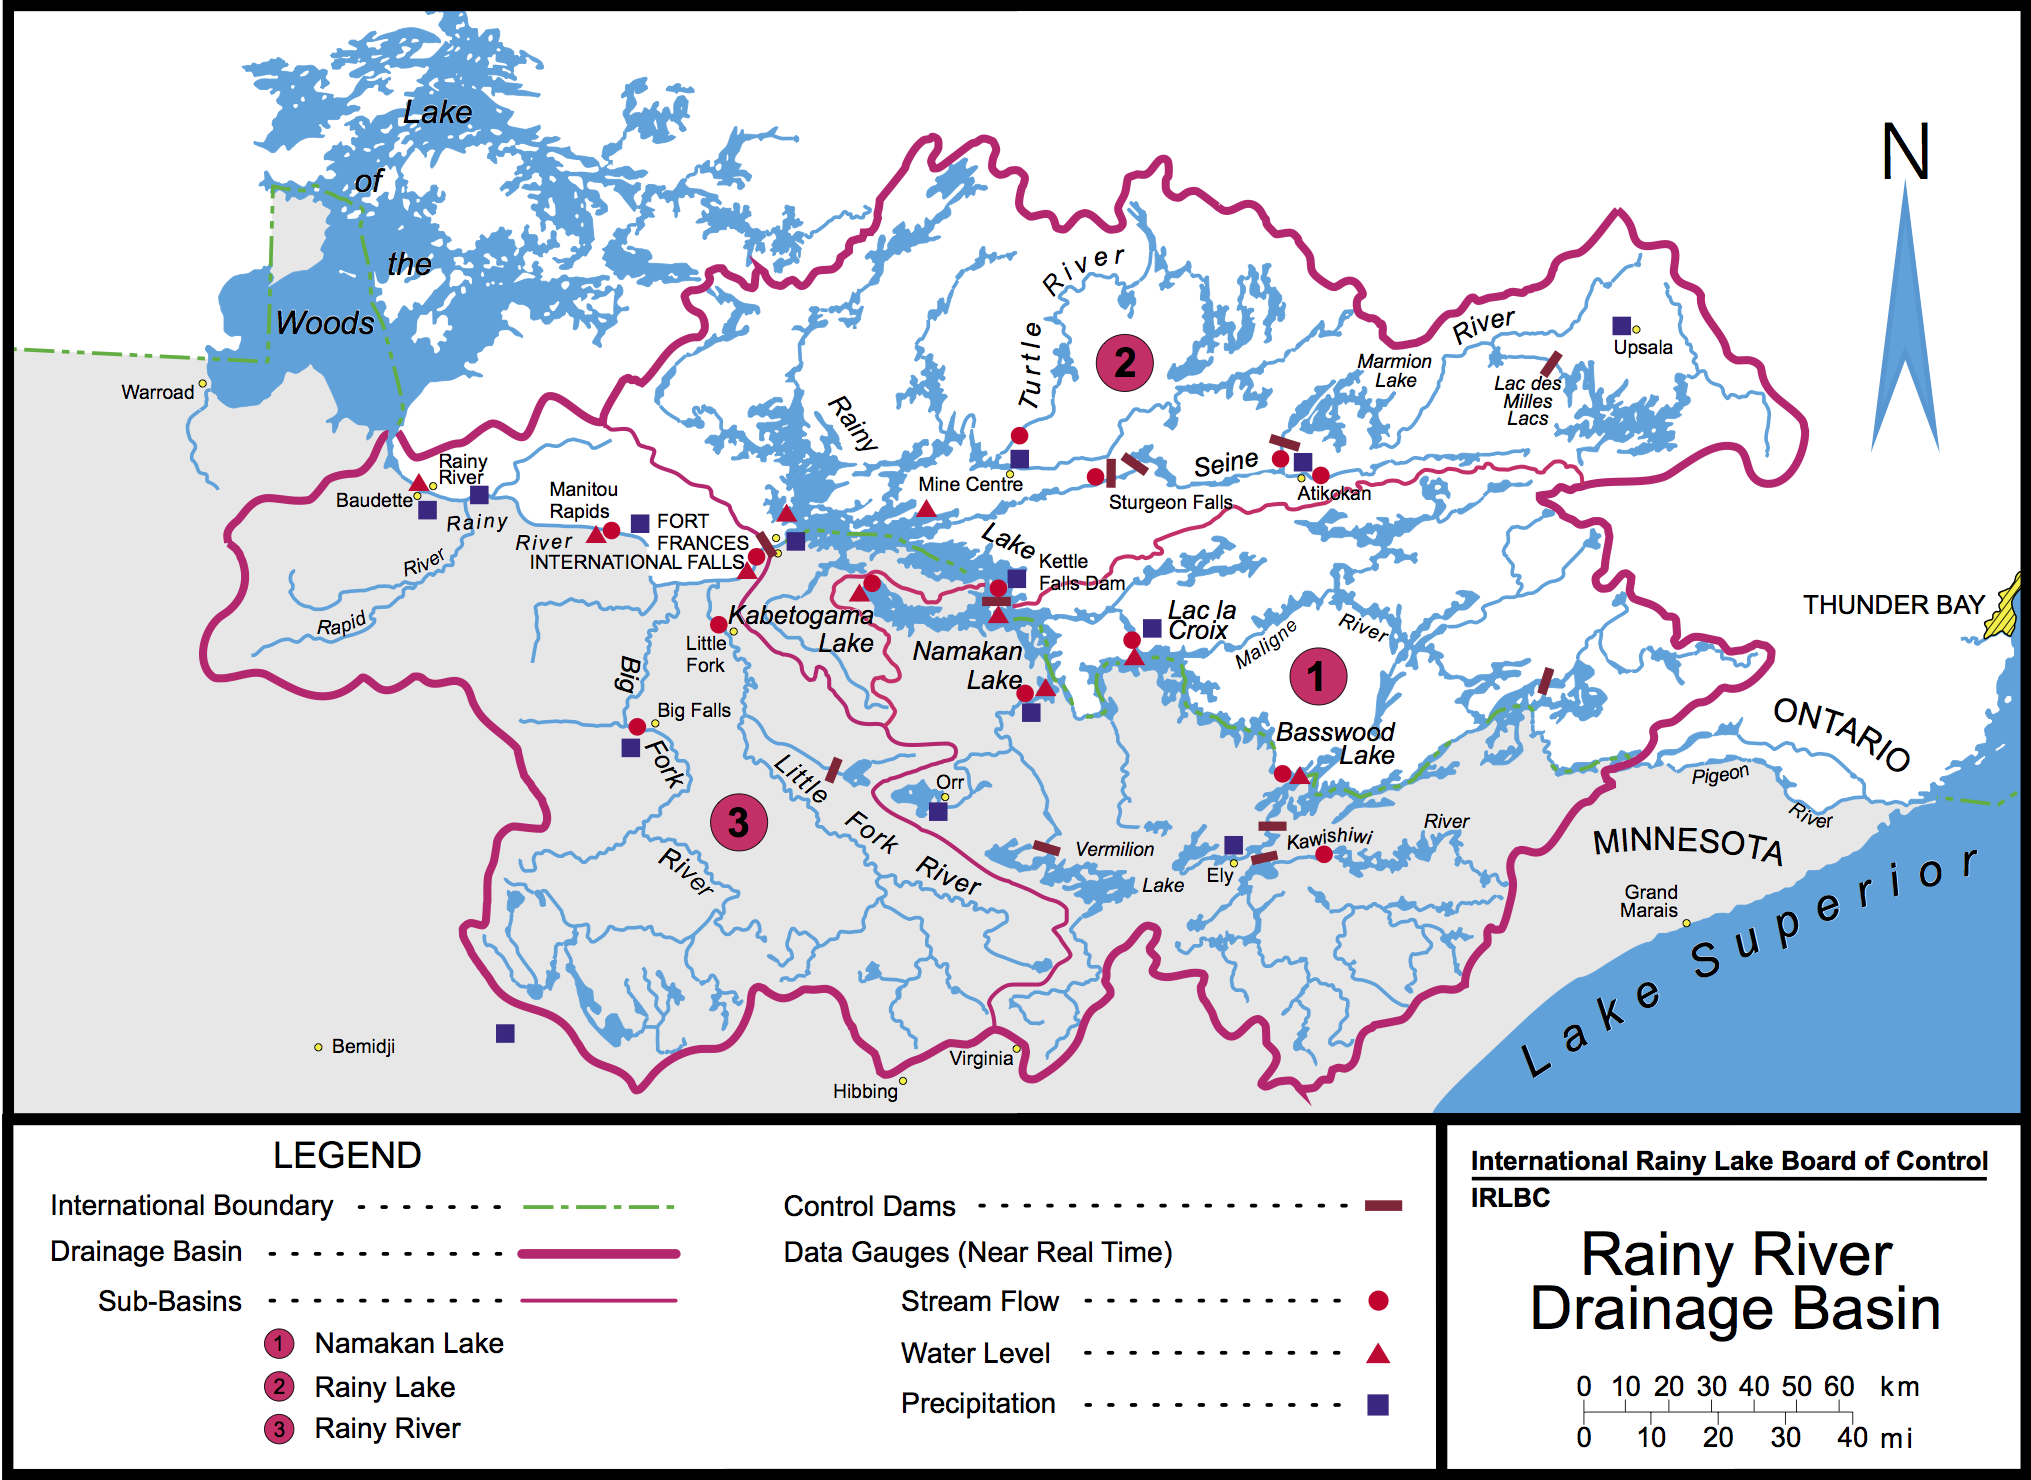
\includegraphics[width=\linewidth]{rl_basinmap.png}
\caption{Map of the Rainy River watershed courtesy of the International Joint Commission. The three major sub-basins are denoted by a red outline. The two control dams considered in this work are located at International Falls, MN/Fort Frances, Ont, and at Kettle Falls. }\label{figure:2}
\end{figure}
 
The Rainy River basin is a complex 55,000+ km$^2$ watershed that is part of the larger Lake of the Woods basin and, ultimately, the Hudson Bay watershed. The Rainy River basin includes Voyageurs National Park, the Boundary Waters Canoe Area (BWCA) and Bois Forte Reservation on the U.S. side of the border, the Quetico Provincial Park wilderness area, and the Mitaanjigamiing, Couchiching, and Nigigoonsiminikaang First Nation communities on the Canadian side. The Rainy River watershed generates revenue through timber for lumber and paper production, electricity generation, recreation, and tourism, and ultimately provides drinking water for 750,000 people downstream.

As part of the trans-boundary waters between the United States and Canada, the Rainy River basin is managed by the binational International Joint Commission created under terms of the Boundary Water Treaty of 1909. The International Joint Commission manages twelve distinct watersheds comprising over 330 lakes and fully 40\% of the 8,800 km border between the US and Canada. 

The primary means of manipulating natural watersheds is through the control of streams flows at the location of control dams. The two largest lakes within the Rainy River watershed, Rainy Lake (approximately 900 km$^2$) and the Namakan Reservoir (approximately, 265 km$^2$) are partially controlled by dams operated by commercial entities under formal Orders issued by the International Joint Commission. Dam operators in this watershed are required to manage lake levels, when feasible, to remain within 'rule curves' that establish upper and lower bounds on lake levels as a function of calendar date. The rule curves include additional specifications and procedures for emergency low and high water conditions. The rule curves specified by the International Joint Commission are a compromise among the interests of stakeholders. The rule curves are periodically reviewed and revised to accommodate ecological, hydrological, economic, and political considerations. The most recent revisions were 1970 and 2000. As of the writing of this manuscript (2017), a review is currently underway that could result in revisions to the standing orders for lake level management, including changes to the rule curves.

The research reported in this paper was initiated following a series of high water events subsequent to the rule curve revision of 2000, including flooding events in the summers of 2002 and 2014. The initial goal of the work was to establish whether the flooding events could have been prevented by improved control of dam operation located on Rainy and Namakan Lakes. Subsequently the project evolved to encompass three main efforts:

\begin{itemize}
\item Development of a tracking filter to estimate net inflows to the major reservoirs in the watershed using available lake level gauges and limited stream flow measurements.
\item Development of multivariable control strategy for the integrated control of the two major dams in the watershed.  Constraints on dam operation include management of emergency high water and low water events, hydrological conveyance constraints upstream of the dams, ecological and property considerations, and constraints on river bank erosion downstream of the dams.
\item Development of a revised rule curve order for the adaptive management of the water levels and flows that is feasible, can accommodate more variable seasonal flows resulting from the effects of climate change, and that accommodate the biological requirements of key sentinel species representative of the regional ecology.	
\end{itemize}

This paper provides an overview of hydrological considerations, estimation of lake inflows from limited sensor measurements, diagnostics, flood prediction and mitigation, and incorporating ecological considerations into predictive control.

\section{System Description}

For the purposes of lake level estimation and control, we consider a simple one-dimensional inventory model of the major lakes in this watershed as illustrated in the accompanying figure. The inventory labelled Namakan Reservoir consists of Namakan Lake, Kabetogama 

\begin{figure}
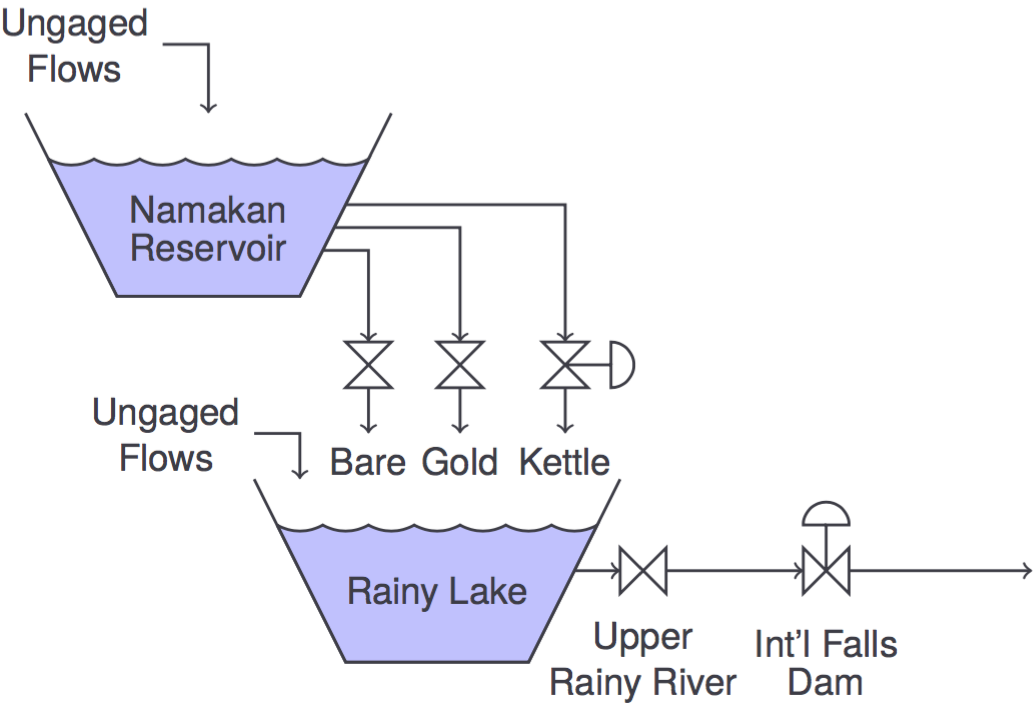
\includegraphics[width=\linewidth]{FlowDiagram}
\caption{The lakes are modeled as simple inventories with level/volume relationships obtained from bathymetry data.}\label{figure:5}
\end{figure}

\section{Estimating Lake Inflows}

A tracking filter was developed for the purpose of estimating the net inflow to Rainy Lake. The filter uses available level gauges and incomplete stream flow data to estimate inflows. The serendipitous occurrence of redundant lake measurements in the historical database provided a statistical model for the level measurement errors. The error model was used to tune the tracking filter to produce maximum likelihood estimates of inflows to Rainy Lake. 

\begin{figure}
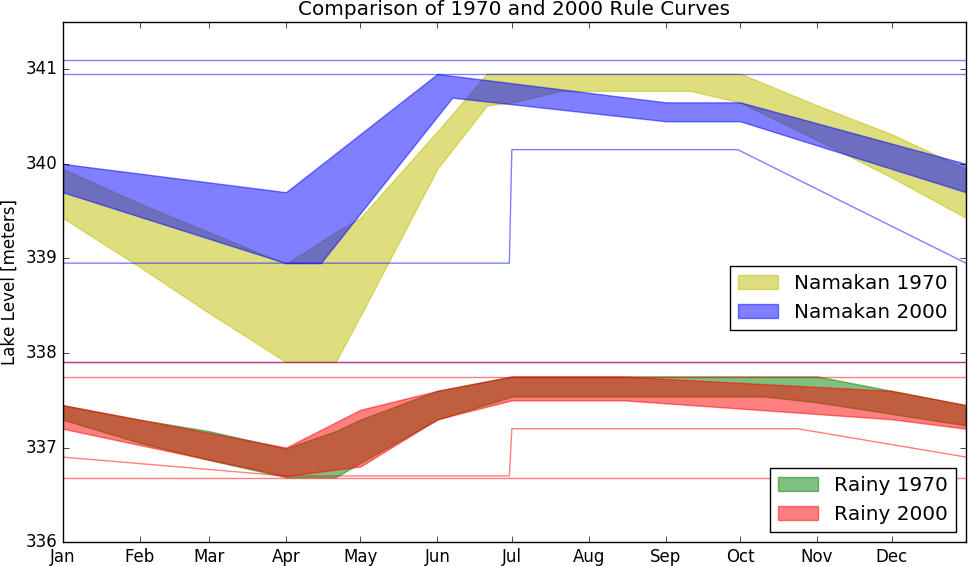
\includegraphics[width=\linewidth]{RuleCurveComparison.png}
\caption{Rule curves establish desired upper and lower bounds of lake levels. This chart compares rules in force for the Namakan Reservoir (upper panel) and Rainy Lake (lower panel) for the period 1970-1999, and 2000 -- present. The additional lines establish emergency high and lower water conditions.} \label{figure:3}
\end{figure}

\begin{figure}
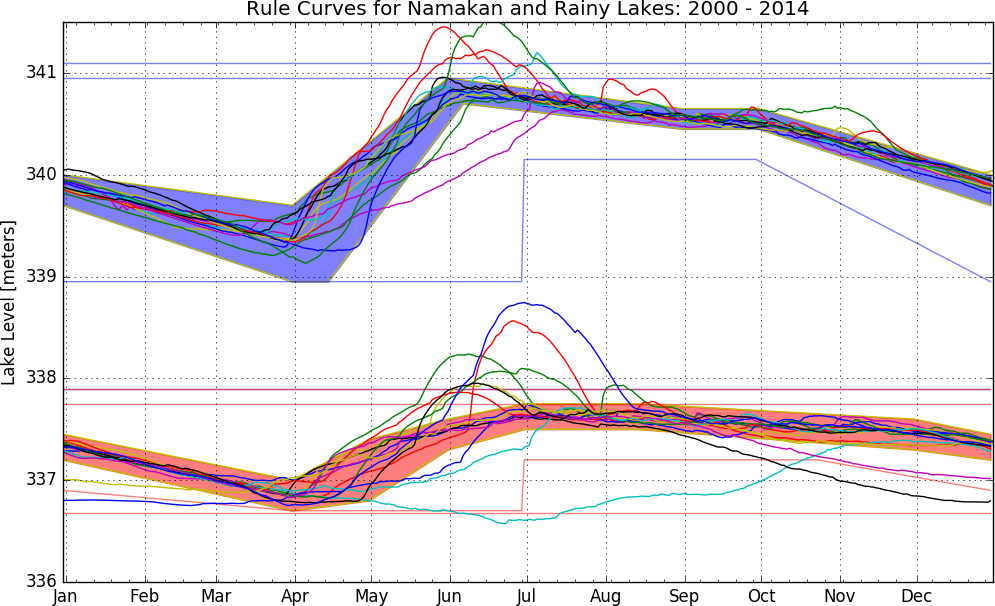
\includegraphics[width=\linewidth]{RuleCurvePerformance2000-2014}
\caption{The levels of Rainy Lake and Namakan Reservoir are compared to the rule curves in effect for 2000-2014. The significant overshoots correspond to flooding events with serious economic and ecological consequences.}\label{figure:4}
\end{figure}

\subsection{Inventory model}

The inventory model assumes the inflows and outflows to Rainy Lake are exogenous disturbances driven by zero mean white noise. The model for daily levels and and daily mean flow is given by

{\tiny
$$\underbrace{\left[\begin{array}{c} H_{RL}(k+1) \\ I_{RL}(k+1) \\ O_{RL}(k+1) \end{array}\right]}_{x(k+1)} = \underbrace{\left[ \begin{array}{ccc} 1 & \frac{\Delta t}{A_{RL}} & -\frac{\Delta t}{A_{RL}} \\0 & 1 & 0\\0 & 0 &  1\end{array}\right]}_{A} \underbrace{\left[\begin{array}{c} H_{RL}(k) \\ I_{RL}(k) \\ O_{RL}(k) \end{array}\right]}_{x(k)} + \underbrace{\left[ \begin{array}{c} 0 \\ w_{I}(k) \\ w_{O}(k)\end{array}\right]}_{w(k)}$$
}

\noindent
where $H$, $I$, $O$ are lake level, inflow, and outflow, respectively. The signals $w_I(k)$, and $w_O(k)$ are zero-mean independent and identically distributed random increments to changing lake inflow and outflows. The vector $w(k)$ is assumed to be distributed as multivariate Normal distribution with zero mean and a covariance $Q$. Lake area $A_{RL}$ depends on lake level, data for which is obtained from lake bathymetry data.

\begin{figure}
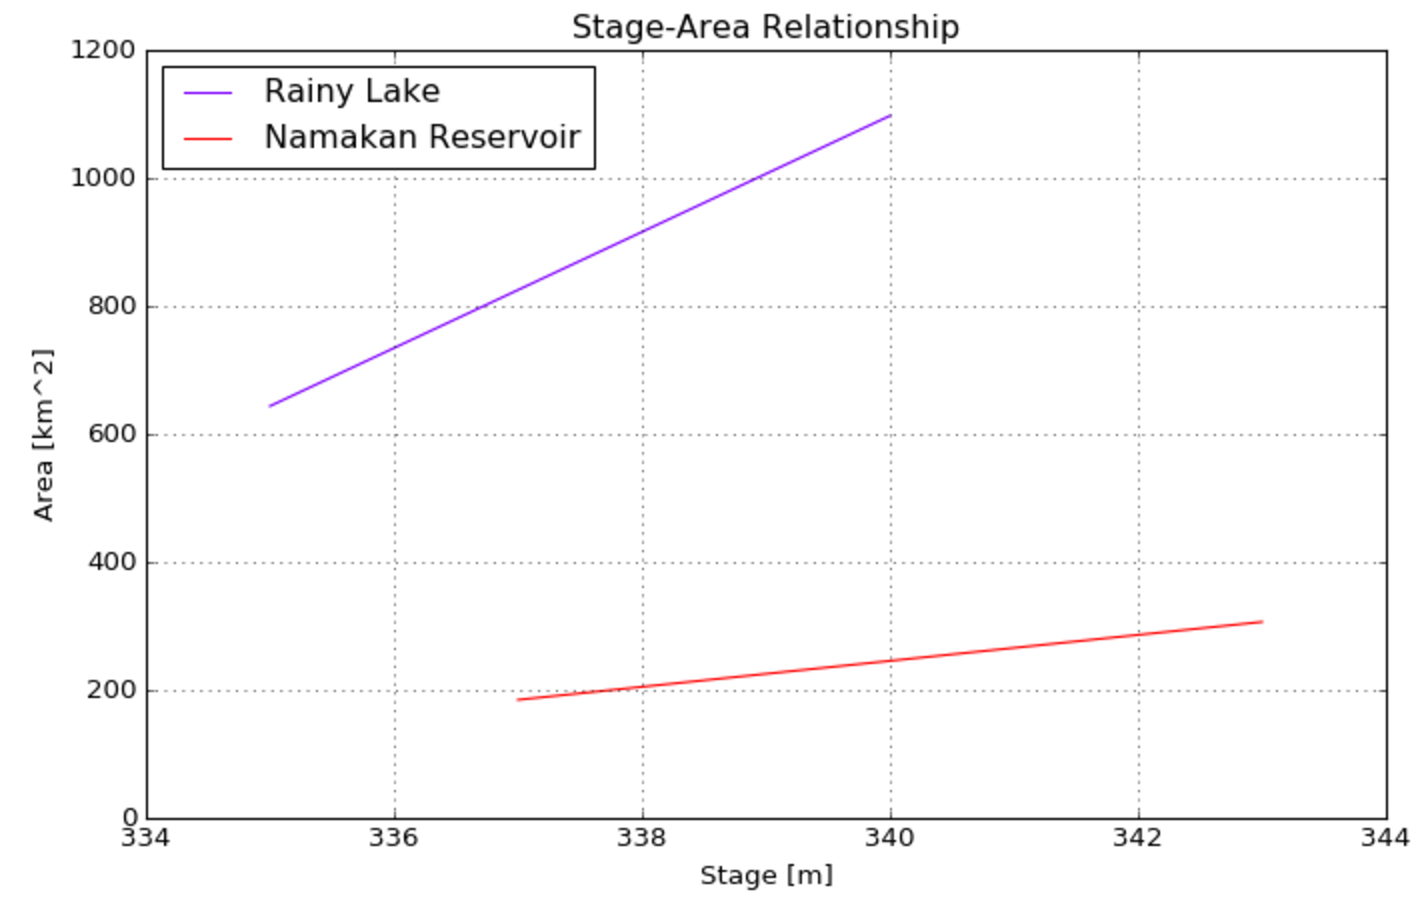
\includegraphics[width=\linewidth]{StageArea}
\caption{Area-Level Relationship for Rainy Lake and Namakan Reservoir.}\label{figure:6}
\end{figure}

The measurement model is written

$$\underbrace{\left[\begin{array}{c} y_H(k) \\ y_O(k) \end{array}\right]}_{y(k)} = \underbrace{\left[\begin{array}{ccc} 1 & 0 & 0 \\ 0 & 0 & 1 \end{array}\right]}_{C} \underbrace{\left[\begin{array}{c} H_{RL}(k) \\ I_{RL}(k) \\ O_{RL}(k) \end{array}\right]}_{x(k)} +  \underbrace{\left[\begin{array}{c}  v_{H}(k) \\ v_{O}(k) \end{array}\right]}_{v(k)} $$

\noindent
where the measurement noise vector $v(k)$ is an i.i.d. random variate with zero mean and a covariance $R$.

A Kalman filter provides a two step method for estimate values of the state vector $x(k)$. The the estimate of $x(k)$ using information up to time $k-1$ is the prediction step given by 

$$\hat{x}(k|k-1) = A \hat{x}(k-1|k-1)$$

\noindent
with covariance

$$\hat{P}(k|k-1) = A \hat{P}(k-1|k-1) A^T + Q$$

In the measurement update step, an innovation is the difference between the actual measurement at time $k$ versus the predicted measurement

$$e(k) = y(k) - C \hat{x}(k|k-1)$$

\noindent
with covariance

$$S(k) = C\hat{P}(k|k-1)C^T + R$$

\noindent
The Kalman filter gain is given by

$$K(k) = \hat{P}(k|k-1)C^TS^{-1}(k)$$

\noindent
which is used to compute the updated state estimate

$$\hat{x}(k|k) = \hat{x}(x|k-1) + K(k)e(k)$$

and covariance

$$\hat{P}(k|k) = \hat{P}(k|k-1) - K(k)S(k)K^T(k)$$

\subsection{Net Inflow to Rainy Lake, 1970-1999 vs 2000-2015}

Historical level for Rainy Lake and outflow data for Rainy River was extracted from the HYDAT Database maintained by the National Water Archive division of the Environment and Climate Change, Government of Canada. Complete code and data files are available on github at \url{https://github.com/jckantor/Rainy-Lake-Hydrology}.

The inflow estimates show a statistically significant change in inflows between the periods 1970-2000 and 2000-2015

\begin{figure}
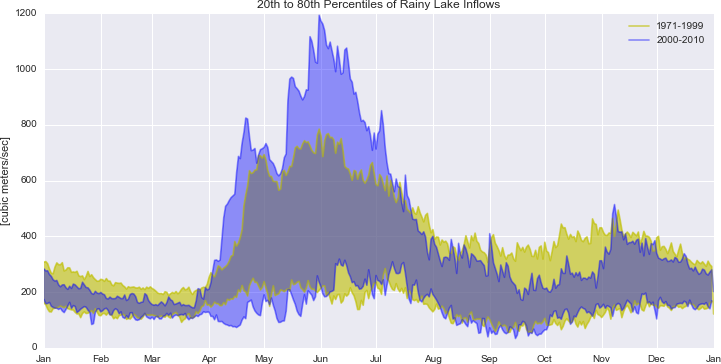
\includegraphics[width=\linewidth]{RainyLakeInflows}
\caption{The 20th to 80th percentiles of inflows to Rainy Lake for the period 1970-1999 vs 2000-2015. The inflows are estimated using a novel tracking filter using lake levels.}\label{figure:7}
\end{figure}

\subsection{Net Inflow to Rainy Lake, 1970-1999 vs 2000-2015}

Historical level for Rainy Lake and outflow data for Rainy River was extracted from the HYDAT Database maintained by the National Water Archive division of the Environment and Climate Change, Government of Canada. Complete code and data files are available on github at \url{https://github.com/jckantor/Rainy-Lake-Hydrology}.

The inflow estimates show a statistically significant change in inflows between the periods 1970-2000 and 2000-2015

\section{Predictive Control}

\subsection{Discharge Characteristics}

The outflow from Rainy Lake is controlled by a power generating dam located approximately 4 kilometers downstream on Rainy River between International Falls, MN, and Fort Frances, ONT. The stretch of river between Rainy Lake and the dam include a rapids and at least two additional constrictions that limit outflow from the lake. 

For the purposes of predictive control, a necessary modeling step is to identify an overall `discharge characteristic' describing the ability of the river and dam to convey water from the lake.

\begin{figure}
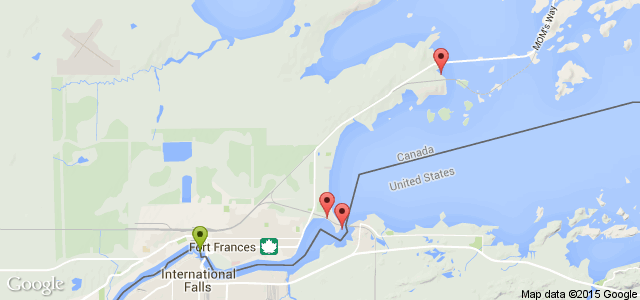
\includegraphics[width=\linewidth]{rlmap}
\caption{Location of level (red marker) and flow (green label) sensors on upper Rainy River. The control dam is located between International Falls, MN, and Fort Frances, ONT.}\label{figure:8}
\end{figure}

The discharge characteristic of upper Rainy River are demonstrated by plotting historical Rainy Lake levels as a function outflow measurements at the dam. Figure \ref{figure:RLdischarge} presents the data coded to distinguish rule curve regimes since 1948. 

The highest levels designated in the plot correspond to 'Emergency High Water' and `All Gates Open (AGO)'. For lake levels below AGO, flow through the dam can be regulated to any level up to the hydraulic capacity of the dam and river. Under the rule curve orders, above the AGO level the dam all gates are opened and the system operated at its full hydraulic capacity. 

\begin{figure}
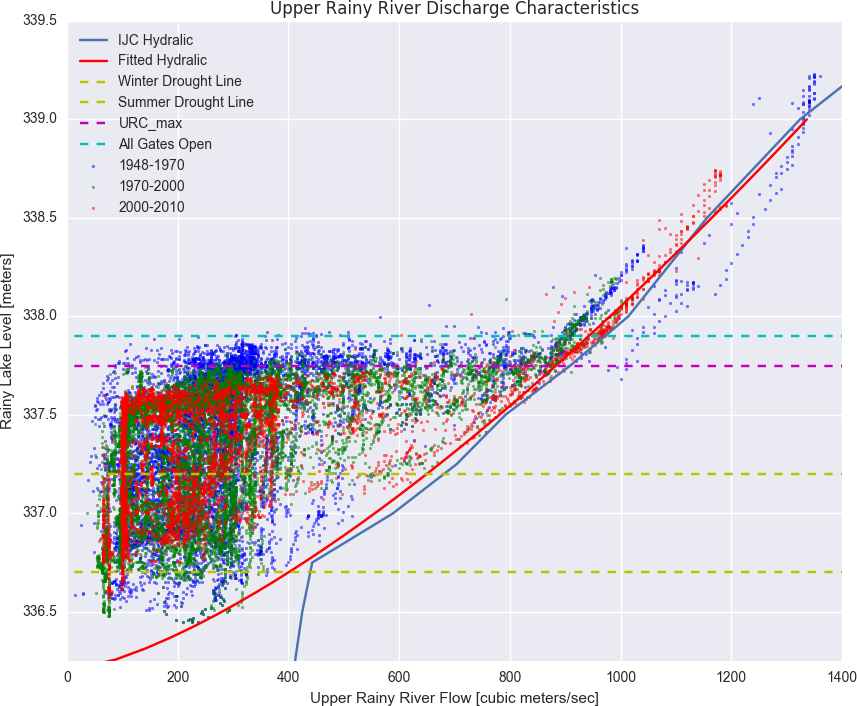
\includegraphics[width=\linewidth]{RainyRiverDischarge_Fit}
\caption{Discharge characteristics of Upper Rainy River color coded by rule curve regime. The fitted red curve denotes the hydraulic capacity of the coupled dam and river system.}\label{figure:RLdischarge}
\end{figure}

For modeling purposes, the dam discharge $O_{RL}$ is modeled as 

$$ O_{RL} = u F(H_{RL}) $$

\noindent
where $H_{RL}$ is lake level, $F(H_{RL})$ is the maximum discharge of the dam established by fitted discharge characteristic in Figure \ref{figure:RLdischarge}, and $u$ is the fractional dam opening.

\subsection{Regulatory Requirements}

The administrative orders for lake level management include a number of explicit requirements that must be incorporated into the control system logic.  The regulatory requirements include:

\begin{enumerate}
    \item All Gates Open. All waste gates for the dam must be opened when water level are higher than the 'All Gates Open' level
    \item Low Water Override. When levels are below low rule curve, flows through the dam to be minimized, but no less than a specified minimum to protect downstream interests.
    \item Emergency Drought Line.  When levels are below the emergency drought line, flows through the dam may be further reduced.
\end{enumerate}

\subsection{Implementation}

\begin{figure}
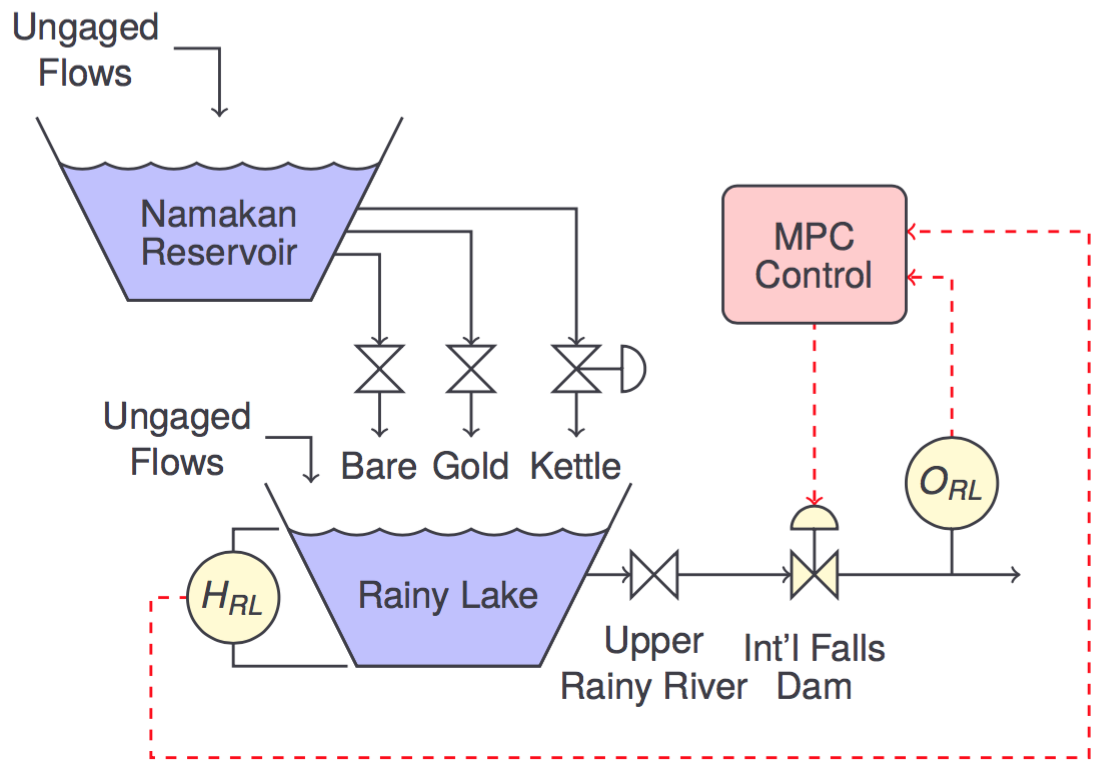
\includegraphics[width=\linewidth]{RLMPC}
\caption{}\label{figure:9}
\end{figure}

A single-loop predictive control strategy was implemented in Matlab/Simulink using the fitted discharge characteristics, level/volume relationship from lake bathymetry, and estimates of historical inflows. 

The basic dam control was computed with an MPC controller targeting the mid-point of the rule curve. A day-of-year schedule provided the rule curve and emergency water level signals. Emergency water level management was implemented as overrides on MPC output, with anti-reset windup used to maintain the internal state of the controller.

\begin{figure}
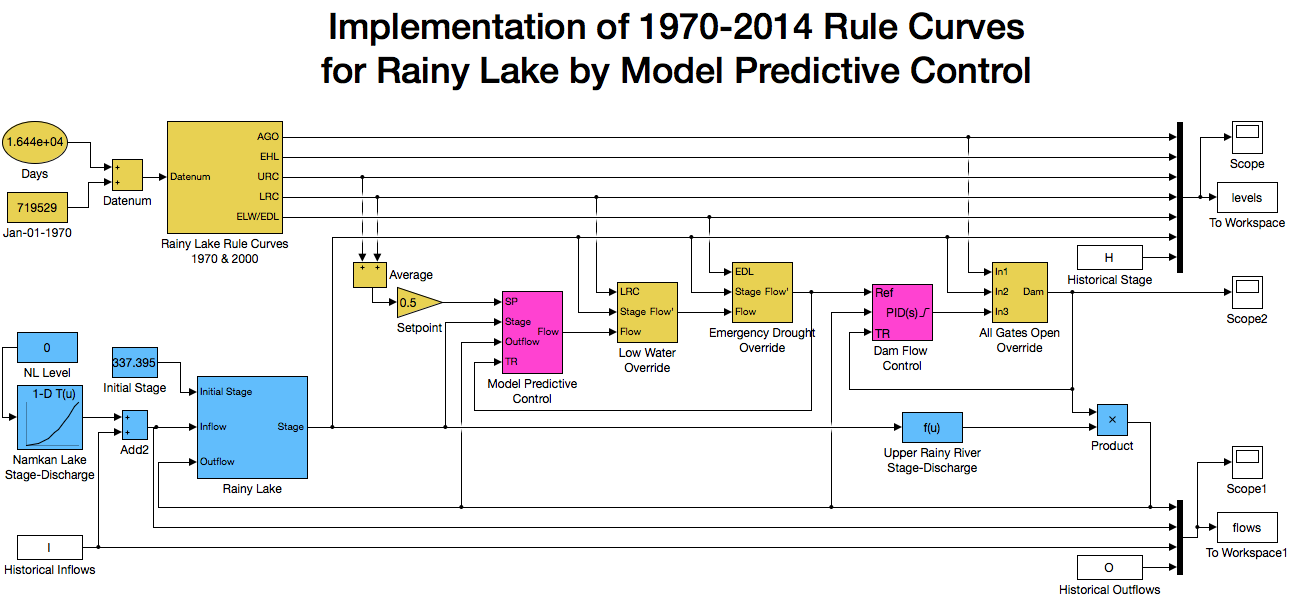
\includegraphics[width=\linewidth]{RLSim_Model}
\caption{A Simulink model for the model predictive control of a power generating dam on Rainy River at International Falls MN/Fort Frances. The model incorporates terms of a treaty regulating dam operation on the international border.}\label{figure:10}
\end{figure}

\begin{figure}
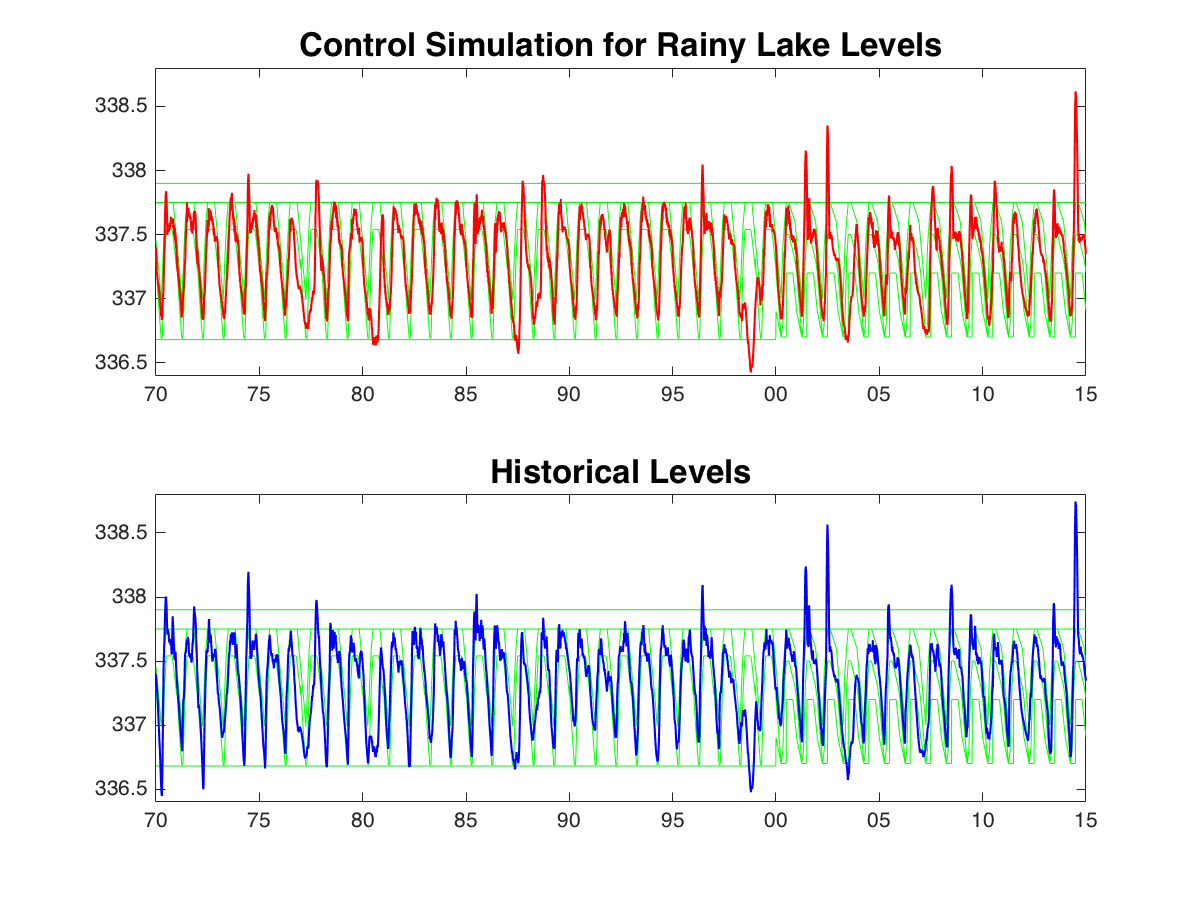
\includegraphics[width=\linewidth]{RLSim_Results}
\caption{Simulated response of Rainy Lake levels to predictive control compared to historical operation. Predictive control reduces the frequency and magnitude of flooding during high water events, and preserves river flow during drought events.}\label{figure:RLSimResults}
\end{figure}

\begin{figure}
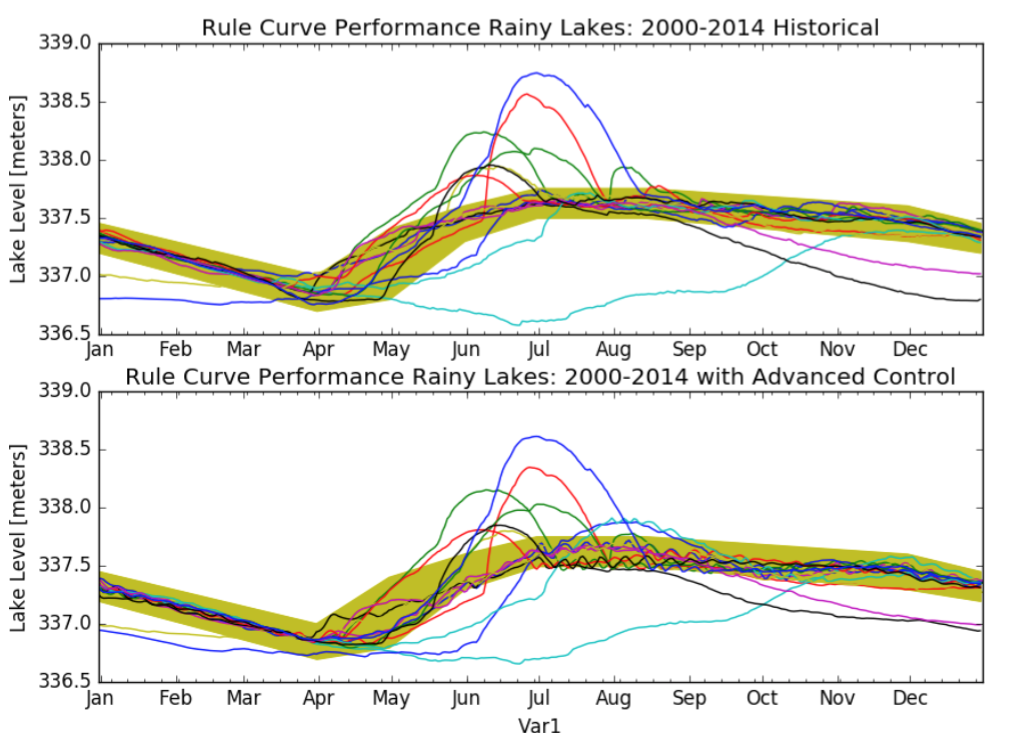
\includegraphics[width=\linewidth]{RLSimResultsA}
\caption{}\label{figure:RLSimResultsA}
\end{figure}

\begin{figure}
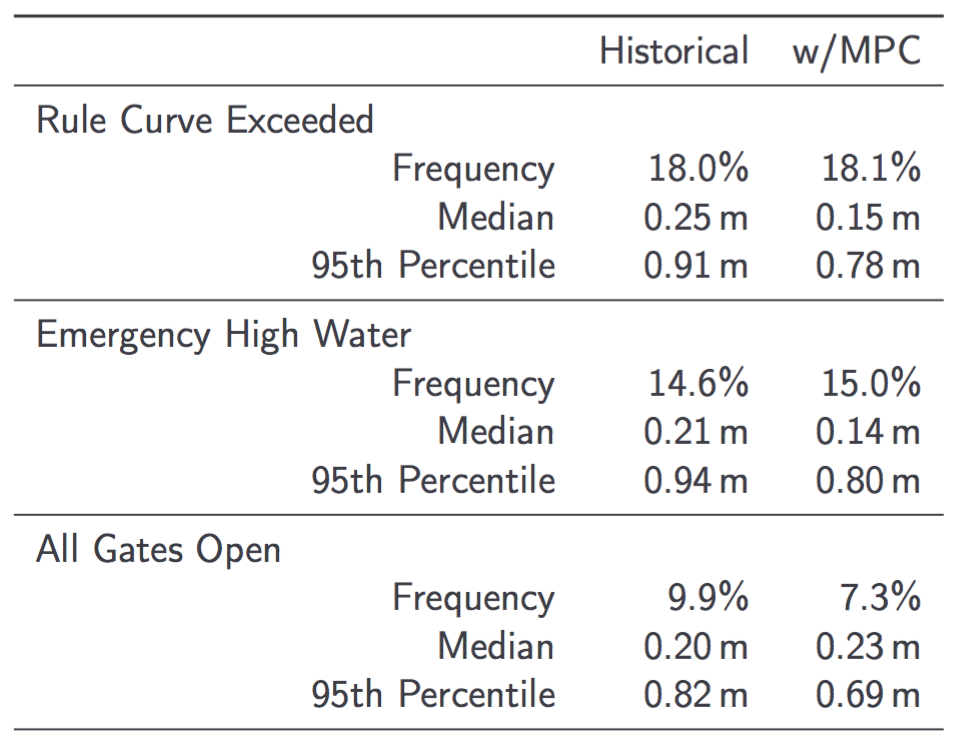
\includegraphics[width=\linewidth]{RLSimResultsB}
\caption{Results of predictive control for Rainy Lake versus historical record for 2000-2014 during the critical May-September high water periods.}\label{figure:RLSimResultsB}
\end{figure}

Performance of the controller compared to historical records is shown in Figures \ref{figure:RLSimResults}--\ref{figure:RLSimResultsB}. The main result is an approximate reduction of 14 centimeters in the 95th percentile of high water events. An unexpected benefit of improved control is a substantial reduction in the number of low water events. These benefits would have substantial but as yet unquantified economic benefits for property owners and businesses operating on the lake.

\begin{figure}
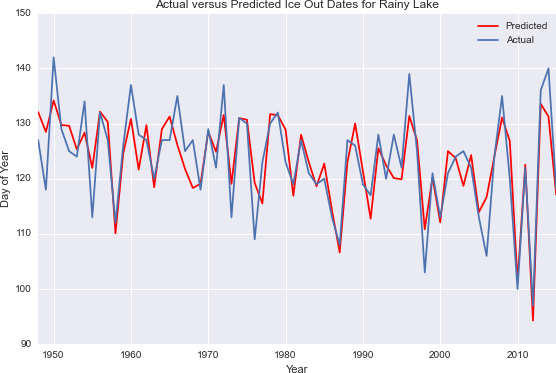
\includegraphics[width=\linewidth]{figures/IceOutPredictor}
\caption{Regression models have been developed to predict the dates of ice-out in the Rainy River basin using winter temperature and precipitation records. The predictor was trained on a limited set of data, and tested against the historical record. This chart compares predicted and observed ice-out dates for historical data.  The ice-out predictor provides a foundation for adapting rule curves to climate change.}\label{figure:11}
\end{figure}

\begin{figure}
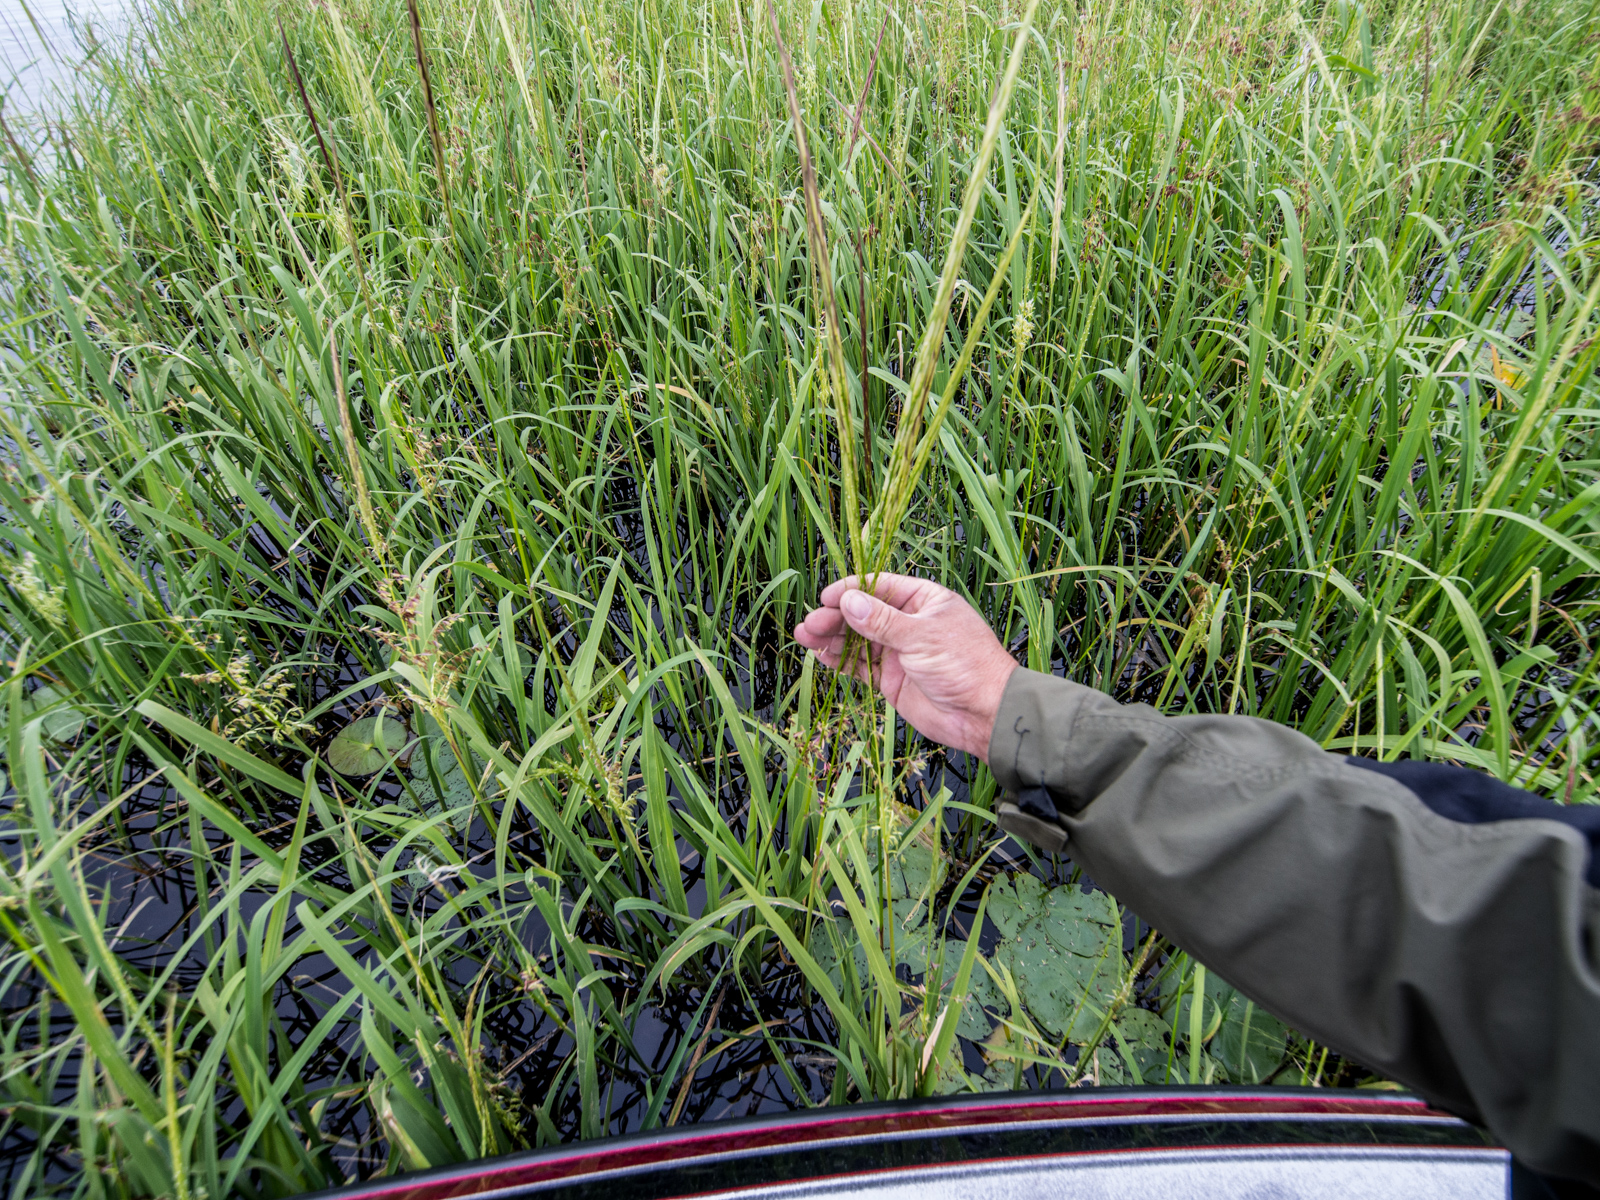
\includegraphics[width=\linewidth]{figures/20150804_194209.jpg}
\caption{Wild rice crop nearing approaching maturity. The success of improved control and adaptive management in the watershed depends on key sentinel species indicative of the regional ecology. In the Rainy River basin these include the wild rice harvested by the First Nations, key fish and waterfowls species, and indicators of invasive species.}\label{figure:12}
\end{figure}

\section{Concluding Remarks}

The primary goal of adaptive management is regulate lake levels and river flows in response to measured events rather than to fixed dates on the calendar. In the Rainy River basin, the change in climate has led to earlier snow melt and ice out of the regions's lakes, and more intense precipitation events in late Spring and early Summer. 

The on-going challenge of this work is to integrate lake level control with the design of rule curves and the management of complex ecosystems. 
\section{Acknowledgements}

The authors received significant advice and background information from numerous sources including Environment and Climate Change Rainy Lake Property Owner's Association, 

\section{References}
\bibliographystyle{apalike}
\bibliography{WatershedControl_CEC}
\end{document}
